\documentclass[a4paper,12pt]{report}
\usepackage[utf8]{inputenc}
\usepackage{graphicx}
\usepackage{titlesec}
\usepackage{adjustbox}
\graphicspath{ {images/} }

\title{Developing a virtual assistant for answering music related questions}
\author{Claudio SCALZO \and Luca LOMBARDO}
\date{v1.0.0}

\begin{document}
	\maketitle
	\tableofcontents

\chapter{Introduction}
	\section{Why a virtual assistant?}
	\section{Scope of the project}
	\section{Expected results}

\chapter{Natural Language Understanding}
	\section{What is NLU?}
	\section{How it works?}
	\section{Advanced techniques (Papers)}
	\section{State of art}

\chapter{Dialogflow}
	\section{What is Dialogflow}
	\section{Why Dialogflow}
	\section{How it works?}

\chapter{DOREMUS}
	\section{What is DOREMUS}
	\section{How is organized}
	\section{How to integrate it in our project}

\chapter{The bot}
	\section{The architecture}
	The architecture of the bot is divided in four categories:
	\begin{center}
		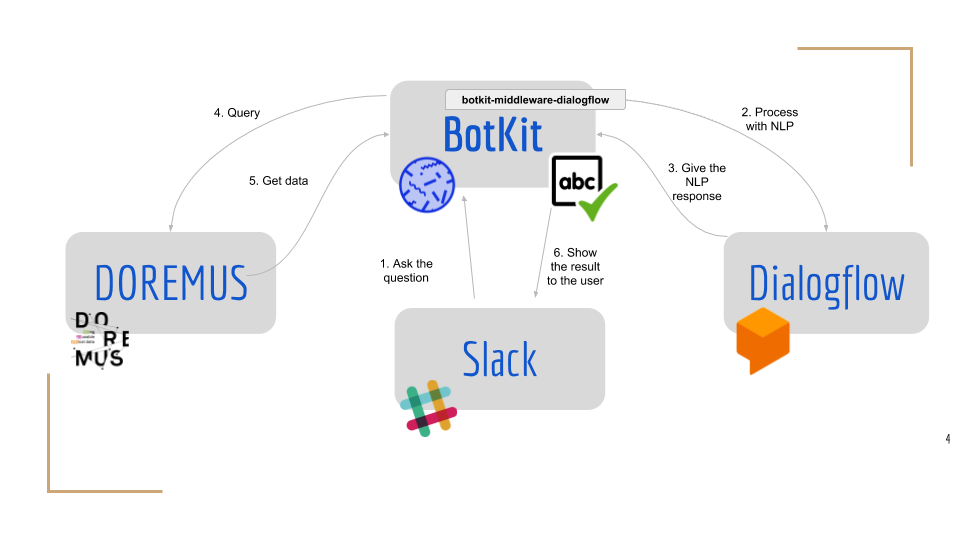
\includegraphics[scale=0.4]{architecture}
	\end{center}
	First of all we can find the client, that in the case of our development, testing and validation process, has been \textit{Slack}. Of course, it can be any of the clients which support the installation of the bot on it (\textit{Telegram}, \textit{Facebook Messenger}, etc.). The use of Slack let us to exploit the beautiful \textit{Slack Cards}, to make the answers of our bot (works, artists, performances) prettier and easier to understand in a glance. A set of examples will be provided in the last chapter.\\\\
	The second part of the architecture is represented by the NLP. In this case, as told in the previous chapter, we used \textit{Dialogflow}, to exploit its advanced slot-filling techniques and its NLU power.\\\\
	However, we didn't use \textit{Dialogflow} on its own, exploiting the direct integration with \textit{Slack}, but we used something that we placed in the middle of the two: \textit{BotKit}. \textit{BotKit} is a bot-making toolkit that aims to ease the building process of a bot, potentially exploiting different NLPs and/or different clients. In our case, \textit{BotKit} has been deployed on a web server, and thanks to the \textit{NodeJS} code we were able to come up with a series of features (like the spell checker) that would have been impossible to reach with a simple (direct) integration between \textit{Slack} and \textit{Dialogflow}. We'll talk more about that in the following paragraphs.\\\\
	The last part of the architecture is of course represented by the data source: \textit{DOREMUS}. We talked about that in the previous chapters, but from the architecture is important to notice how the knowledge base is queried: each query is dynamic, in the sense that according to the intent, the number of filters and the desired results wanted by the user, the query will have a different shape and a different content. The code in the web server is able to add different pieces of queries according to what \textit{Dialogflow} is able to understand and to provide as output values of the API.
	\section{Intents}
	\section{The flow}
	\section{The spell checker}

\end{document}          
